\section{\texorpdfstring{\Gls{spade}}{SPADe} flow}
\label{sec:ch7_designFlow}

\begin{figure}[t]
\centerline{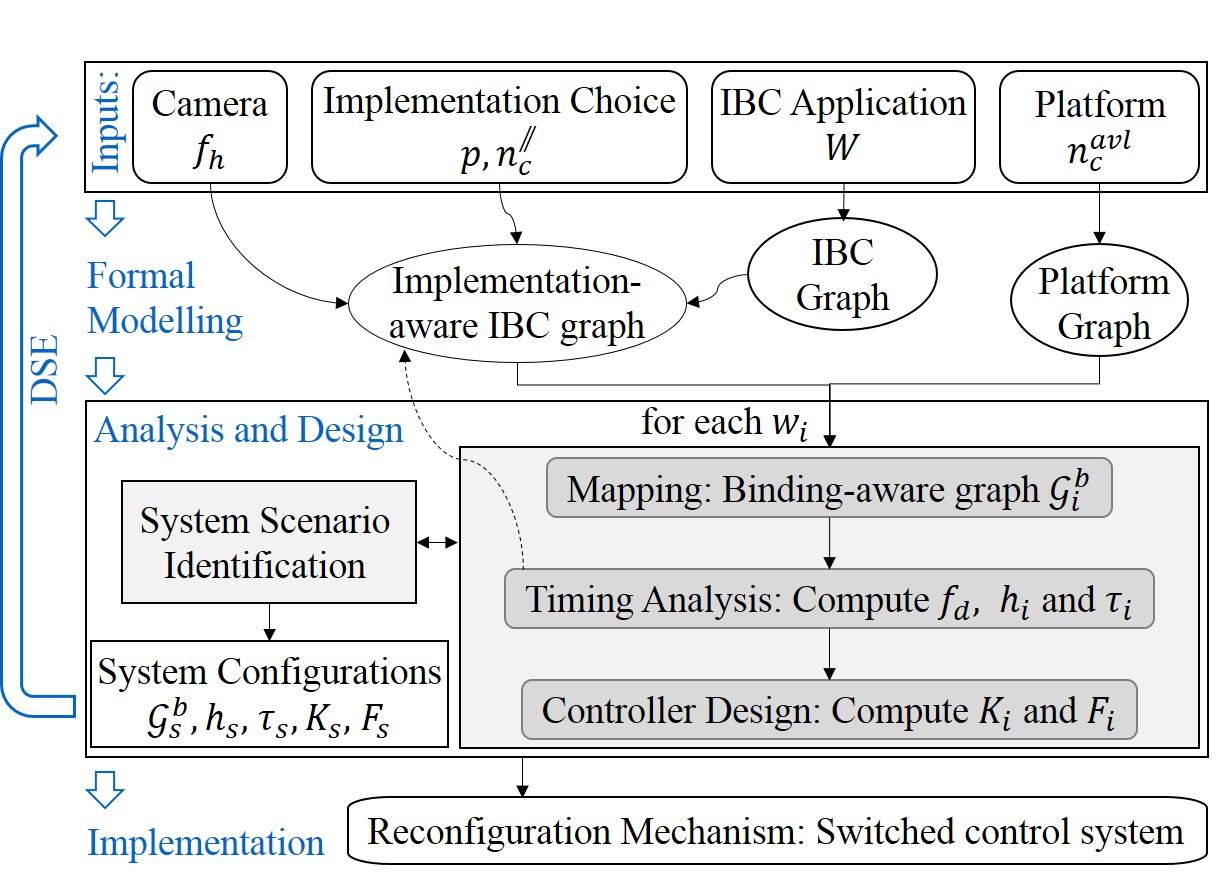
\includegraphics[width=\textwidth]{images/SPADeOverview5.jpg}}
%\vspace{-1ex}
\caption{Overview of our \gls{spade} design flow (repeating Fig.~\ref{fig:ch1_spade_overview}, for readability). $\setW$ is the set of varying workloads and $\workloadScenario,\ \bindingAwareSDFG{i},\ \tau_i,\ h_i, \Kgain_i$ and $\Fgain_i$ are the workload, binding-aware graph, sensor-to-actuator delay, sampling period, feedback gain and feedforward gain for a workload scenario $\workloadScenario$ (determined by $\workloadScenario\in\setW$); 
$\bindingAwareSDFG{s},\ \tau_s,\ h_s, \Kgain_s$ and $\Fgain_s$ are the corresponding parameters for an identified system scenario $\sysScenario$ (that abstract multiple workload scenarios). $\fh$ is the camera frame arrival period, $\fd$ is the inter-frame dependence time, $\numPipes$ is the number of pipes for pipelining, $\numCoresParallel$ is the number of cores allocated for parallelism per pipe, and $\numCoresAvailable$ is the total number of available cores.}
\label{fig:ch7_ibc_overview}
\end{figure}

We present the \gls{spade} for \gls{ibc} systems extending the approach presented in Chapter~\ref{chap:parallelisation} by considering pipelining along with parallelism and formalising the \gls{ibc} system modelling.
An overview of our \gls{spade} approach is illustrated in Fig.~\ref{fig:ch7_ibc_overview} (repeating Fig.~\ref{fig:ch1_spade_overview}, for readability), summarised below and explained in detail in subsequent subsections.

\begin{enumerate}
    \item Formal modelling of the \gls{ibc} system: An \gls{ibc} application is captured as an \gls{ibc} \gls{sadf} model considering workload variations $\setW$ and the platform as a platform graph. Further, an \emph{implementation-aware} \gls{ibc} \gls{sadf} model captures the given design parameters - camera frame arrival period $\fh$, maximum number of allowed pipes $\numPipes$, total number of available cores $\numCoresAvailable$ and allocated processing cores for parallel execution per pipe $\numCoresParallel$.
    The design parameters fully determine the implementation choice - non-pipelined without parallelism, non-pipelined with parallelism, pipelined without parallelism and pipelined with parallelism. The parallelism here refers to the parallel execution of sensing subtasks limited by the degree of parallelism of the \gls{ibc} application.
    Graph transformations are proposed to obtain the implementation-aware \gls{sadf} model.
    \item Analysis and design: We map the implementation-aware \gls{ibc} graph for each workload $\workloadScenario \in \setW$ to the platform graph to obtain the \emph{binding-aware graph} $\bindingAwareSDFG{i}$ for that specific workload using the SDF3 mapping flow~\cite{stuijk2007}. 
    $\bindingAwareSDFG{i}$ is a \gls{sdfg} that models the mapping of the implementation-aware graph to the platform graph. The mapping binds each actor in the \gls{sdfg} to a processing core in the platform graph. For the ordering of execution of actors bound to the same core, a static-order schedule is encoded in the \gls{sdfg}.
    A throughput and latency analysis of $\bindingAwareSDFG{i}$ yields the sensor-to-actuator delay $\tau_i$, and sampling period $h_i$.
    For a pipelined implementation, the throughput analysis of the worst-case image-workload scenario allows to compute the inter-frame dependence time $\fd$ (as explained later in Section~\ref{sec:ch7_IFD}). 
    If $\fd>h_i$, the implementation-aware graph is updated with the realisable period and $\tau_i$ and $h_i$ are recomputed. 
     The controllers are then designed for the resulting $(\tau_i,\ h_i)$ to obtain the controller feedback and feedforward gains $(\Kgain_i,\ \Fgain_i)$.
     Trying to cater to the designed workload scenarios at runtime means that we have a switching system. A switching system with too many switching states is challenging for controller stability and may result in poor performance. 
     Hence, we aggregate multiple workload scenarios with similar control timing parameters as a \emph{system scenario}.
    A system scenario $\sysScenario$ abstracts multiple workload scenarios and has a constant $(\tau_s,\ h_s)$ during implementation. A \emph{system configuration} is defined as the combination of mapping and controller configurations, i.e. $\bindingAwareSDFG{s}$, $\tau_s,\ h_s,\ \Kgain_s,$ and $\Fgain_s$ (as explained later in Section~\ref{sec:ch7_sysConfigStability}).
    Typically, there are a few identified system scenarios, and the idea is that switching between the system scenarios at runtime guarantees stability and improved performance.
    For pipelined parallelism, a \gls{dse} using the \gls{spade} flow needs to be performed by varying the design parameters to identify the best implementation choice (parameters $\numPipes, \numCoresParallel$, further explained in Section~\ref{sec:ch7_DSE}).
    \item Runtime implementation: The system configurations for the implementation choice are stored in a \gls{lut} in platform memory for the runtime implementation. Dynamic runtime reconfiguration may be needed since there can be a switching behaviour between system configurations due to image-workload variations.
\end{enumerate}

\subsection{Formal modelling}
%\label{sec:ch7_FormalModelling}
An \gls{ibc} application is captured as an \gls{ibc} graph considering workload variations and the platform as a platform graph. 
Further, an \emph{implementation-aware} \gls{ibc} graph is created considering the design parameters (the number of pipes $\numPipes$, allocated processing cores for parallel execution per pipe $\numCoresParallel$ and camera frame arrival period $\fh$).

\subsubsection{\Gls{ibc} graph and implementation-aware graph}
\label{sec:ch7_IBCGraph}
The \gls{ibc} and implementation-aware graphs are modelled using an \gls{sadf} model.
Graph transformations to obtain an implementation-aware graph from the \gls{ibc} graph are different for the different implementation choices and, as such, are explained in later sections.
We choose \gls{sadf}~\cite{theelen2006scenario} as the formal \gls{moc} for our application as it enables us to: i) model dynamic behaviour and dependencies, analyse timing, and optimally map application (sub)tasks to the platform for maximising the effective utilisation of allocated resources; 
ii) relate latency and throughput of the dataflow graph to the control timing parameters $\tau$ and $h$, and thus combine dataflow analysis and mapping with control design parameters and \gls{qoc}; 
iii) analyse inter-frame dependencies (captured as inter-frame dependence time $\fd$) through graph transformations (as explained in Section~\ref{sec:ch7_ModelTransformations});
and iv) to efficiently implement a runtime mechanism that manages necessary dynamic reconfiguration.

\begin{figure}
    \centering
    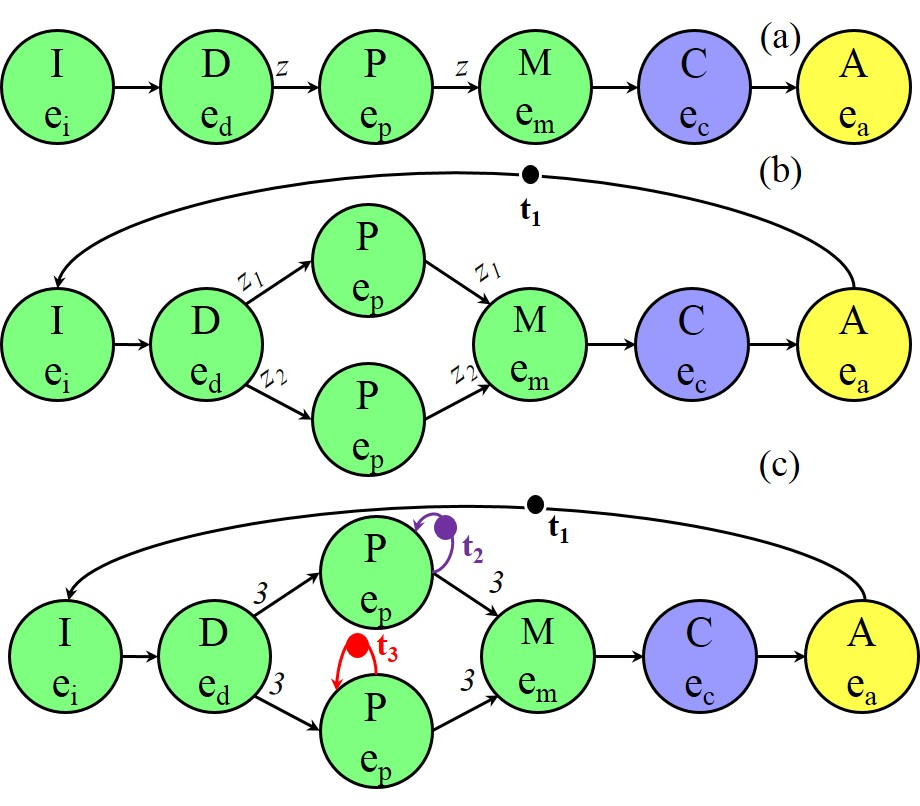
\includegraphics[width=0.7\textwidth]{images/modelGraphs.jpg}
    \vspace{-1em}
    \caption{\Gls{ibc} \gls{sdfg}: (a) graph structure. The rates $\rateY$ indicate the workload $\setW$. (b) Implementation-aware graph for non-pipelined implementation on two cores (given platform allocation). (c) A (simplified) binding-aware graph for non-pipelined implementation on two cores for a workload of 6 \gls{roi}. 
}
    \label{fig:ch7_SADF}
\end{figure}
An \gls{sadf} model is a tuple ($\Scenarios,\ \fsmsadf$) of scenarios $\Scenarios$ and scenario sequences $\fsmsadf$, as already explained in Section~\ref{sec:ch5_sadf}.
The \gls{sadf} model for our example \gls{ibc} system is visualised in Fig.~\ref{fig:ch7_SADF}~(a). It is a variant of the model already used in Chapter \ref{chap:parallelisation}, with an explicit image-signal preprocessing step and shorter actor names.
The sensing and processing task receives the RAW camera image frames, which are processed in a sequence of steps to extract the state information required for the controller. 
The image-signal (pre-)processing (\taskISP) subtask converts the RAW image in the Bayer domain to pixels in the RGB domain. \mbox{(Sub-)}tasks translate to actors in the dataflow graph, shown as circles in the figure. Data dependencies between \mbox{(sub-)}tasks translate to channels, shown as arrows.
After the image processing, we detect the \glspl{roi} in the RGB image frames (\taskRoID). \Gls{roi} are processed (\taskRoIP), and, subsequently, the controller state (the lateral deviation $\yL$ in our \gls{lkas} case study) is computed by the \gls{roi} merging (\taskRoIM) subtask. The control algorithm (\taskC) then computes the controller input $u[k]$ (steering angle $\delta_f$ in our \gls{lkas} case study) and feeds it to the actuation (\taskA) task.
The total number of \gls{roi} detected by \taskRoID\ determines the workload $\aWorkload_i$, i.e., $\aWorkload_i=\rateY$ in Fig.~\ref{fig:ch7_SADF}~(a).
The workloads translate to variable token production and consumption rates in the graphs.

Graph transformations are required to analyse the parallel and/or pipelined implementations.
This is, among others, because the typical mapping analysis tools assume that one actor can be bound to only one processing core.   Fig.~\ref{fig:ch7_SADF}~(b) shows an implementation-aware graph for a non-pipelined parallelised implementation on two processors. It has two actor instances of the \taskRoIP\ subtask. The workload $\aWorkload_i=\rateY_{1}+\rateY_2$ in this case.

Each workload $\aWorkload_i$ in an \gls{sadf} is associated with an \gls{sdfg} $\SDFG_i$. 
An \gls{sdfg} instance of Fig.~\ref{fig:ch7_SADF}~(b) is obtained by assigning values to parameters $\actorET_j$ (the actor execution times) and $\rateY_k$. 
E.g., assigning $\rateY_1=3,\ \rateY_2=3,\ \actorET_i=10,\ \actorET_d=5,\ \actorET_p=10,\ \actorET_m=3\times(\rateY_1+\rateY_2)=18,\ \actorET_c=1,\ \actorET_a=1$ gives the \gls{sdfg} for a workload of 6 \gls{roi} for mapping to two processors.
There is one (labelled) initial token $t_1$ in the channel from actor \taskA\ to \taskISP. This channel, with its single initial token, enforces a non-pipelined execution of the control loop. 
All actors in Fig.~\ref{fig:ch7_SADF}~(a) have repetition-vector entries of 1, except actor $\taskRoIP$, which as a repetition-vector entry $z$; and all actors in Fig.~\ref{fig:ch7_SADF}~(b) have repetition-vector entries of 1, except the two $\taskRoIP$ instances that have entries $z_1$ and $z_2$ respectively.

Fig.~\ref{fig:ch7_SADF} does not show the language of allowed scenario sequences. In the \gls{lkas} case, all possible workload sequences are allowed.

\subsubsection{Platform graph}
%\label{sec:ch7_platformGraph}
A platform, e.g.\ the \gls{compsoc} \gls{mpsoc} shown in Fig.~\ref{fig:mpsoc}, is modelled as a platform graph that captures processing resources, and other relevant aspects such as memories and connections, with their processing and access latencies, data rates, etc. The details needed for the model depend on the used mapping flow.
For the sake of explaining \gls{spade}, we assume the platform is simply abstracted as a set of tiles.
A tile $\tiles_i$ abstracts a resource with the processor type $pt_i$ that determines the execution time of actors bound to the tile.
The \gls{compsoc} instance shown in Fig.~\ref{fig:mpsoc} has three tiles. Two of these tiles have a microblaze processor type. The third tile is a memory tile that does not play a role in further explanations. Also, the connections are abstracted for the sake of simplicity. Hence, the platform is abstracted as a 2-node platform graph without any connections. Note that the used SDF3 mapping flow does support the modelling of memories and connections, including their timing, and takes these into account in the mapping optimisation. 

A platform allocation determines the resources that are allocated to a task or to an application. 
Resources that are allocated may include the number of tiles or processors, or parts of processors (e.g.\ slots in a \gls{tdm} frame in \gls{compsoc}), and types of processors, e.g. \gls{gpu}, ARM, and microblaze. For our running \gls{lkas} example, an allocation consists only of the number of tiles of a specific processor type. 

\subsection{Analysis and design}
We map the implementation-aware \gls{ibc} graph for each workload $\aWorkload_i\in \setW$ to the platform graph to obtain the \emph{binding-aware graph} $\bindingAwareSDFG{i}$ (further explained below) using the SDF3 mapping flow~\cite{stuijk2007}. 
A throughput and latency analysis of $\bindingAwareSDFG{i}$ yields the control timing parameters $\tau_i$ and $h_i$ for the workload scenario $\workloadScenario$. Controllers are designed for each workload scenario $\workloadScenario$ using the computed timing parameters $(\tau_i,\ h_i)$ to obtain the controller feedback and feedforward gains $(\Kgain_i,\ \Fgain_i)$. System-scenario identification is then performed to identify the set of system scenarios for runtime implementation. 
For a pipelined implementation, inter-frame dependence time $\fd$ (as explained in Section~\ref{sec:ch7_IFD}) is also computed using the throughput analysis.

\subsubsection{System mapping and mapping configurations}
System mapping refers to the mapping of the \gls{ibc} application (modelled as an \gls{sadf}) to the given platform (modelled as a platform graph). 
Note that for each workload scenario $\workloadScenario$, we can have multiple mapping options for the given platform allocation. 
The throughput and latency of each of these mapping options would be different.
The concrete problem is to find the mapping of $\workloadScenario$ to the given platform allocation that maximises throughput.
Any design flow that does the (Pareto-)optimal mapping of an application to a platform while maximising throughput can be used. 

We use the SDF3 mapping flow~\cite{stuijk2006sdf} as it optimises the resource usage, memory load and communication load for mappings (to the extent that these aspects are considered in the models), and embeds state-of-the-art throughput analysis techniques.
Mapping an $\scenario_i$ (modelled as an \gls{sdfg} $\SDFG_i$) to a platform graph generates a binding-aware \gls{sdfg} $\bindingAwareSDFG{i}$.
$\bindingAwareSDFG{i}$ is an \gls{sdfg} that models the mapping of the implementation-aware graph to the platform graph, where each actor in the \gls{sdfg} is bound to a tile in the platform graph. For the ordering of execution of actors bound to the same tile, a static-order schedule is encoded in $\bindingAwareSDFG{i}$.

Fig.~\ref{fig:ch7_SADF}~(c) shows a simplified binding-aware graph for the 6-\gls{roi} workload scenario of the running example, bound to two tiles. It encodes two static-order schedules: \taskISP\taskRoID\taskRoIP$^3$\taskRoIM\taskC\taskA\ for one iteration of the graph on one core and \taskRoIP$^3$ for one graph iteration on the second core. Self-loops with a single token need to be added to the two parallelised \taskRoIP\ actors to model the binding of the actor to a particular core and to enforce sequential execution of the \taskRoIP\ firings on each of the two cores. This suffices to encode the schedules. The graph is simplified in the sense that SDF3 encodes many more aspects in the binding-aware graph, such as memory accesses and interprocessor communication. 

A \emph{mapping configuration} $\Configuration_{\workloadScenario}^m$ refers to the binding of $\workloadScenario$ to the platform and its execution schedule represented in a binding-aware \gls{sdfg}.
The \gls{spade} flow tries to minimise the number of cores used even if a given number of cores is allocated. This happens naturally when we map our \glspl{sdfg} to the platform using the SDF3 tool, as SDF3 gives a Pareto-optimal mapping that minimises utilisation.

\subsubsection{Timing analysis - computing $\fd, \tau_i$ and $h_i$}
%\label{sec:ch7_timingAnalysis}
The computation of inter-frame dependence time $\fd$ is specific for pipelined implementation and is explained later in Section~\ref{sec:ch7_IFD}. In this subsection, we explain how we compute the throughput and latency of the \gls{sadf} and relate it to the control timing parameters $\tau_i$ and $h_i$ for a workload scenario $\workloadScenario$.
Note that the state-of-the-art \gls{sadf} analysis uses (max, +) algebra~\cite{baccelli1992synchronization} and the definitions needed for the computation of throughput have already been explained in Chapter~\ref{chap:parallelisation}.
In this subsection, we summarise the relevant definitions for our analysis.
 For detailed explanations, the reader is referred to~\cite{ara2018scalable}.

A time-stamp vector $\maxplusLambda{0}{}$ captures the availability times the initial tokens.
The production times of the final tokens resulting from the execution of a scenario $\scenario$ are then $\maxplusLambda{1}{} = \maxplusMatrix_{\scenario} \maxplusLambda{0}{}$, where $\maxplusMatrix_{\scenario}$ is the scenario (or state) matrix of $\scenario$.
For the binding-aware scenario \gls{sdfg} corresponding to 6 \gls{roi}, introduced in Fig.~\ref{fig:ch7_SADF}~(c), 
$\maxplusLambda{0}{}=\left[ 0\, 0\, 0\right]^T$. That is, the three initial tokens are all available at time 0. Scenario matrix $\maxplusMatrix_{\scenario}$ captures the dependencies and corresponding delays between the initial and final tokens. For the running example, $\maxplusMatrix_{\scenario}$ equals

{\small
$$
    \begin{bmatrix}
    \actorET_i+\actorET_d+3\actorET_p+\actorET_m+\actorET_c+\actorET_a & \hspace*{-1mm}\actorET_m+\actorET_c+\actorET_a & \hspace*{-1mm}\actorET_m+\actorET_c+\actorET_a \\
    \actorET_i+\actorET_d+3\actorET_p & 3\actorET_p & -\infty{} \\
    \actorET_i+\actorET_d+3\actorET_p & -\infty & 3\actorET_p \\
    \end{bmatrix}
$$
}

Entry $ij$ in this matrix contains the time delay from consuming token $t_j$ to reproducing token $t_i$ in one iteration of the graph. The top left entry thus indicates the delay to reproduce the final token $t_1$ on the \taskA-\taskISP\ channel. The two $3\actorET_p$ entries show that the three firings of the two \taskRoIP\ actors are sequentialized. The two $-\infty$ entries indicate that the two self-loop tokens of the two \taskRoIP\ actors, $t_2$ and $t_3$,  are independent. The other entries capture the delay from $t_1$ to the self-loop tokens $t_2$ and $t_3$ and the delay from $t_1$ to $t_2$ and $t_3$.

With the concrete actor execution times given earlier, this results in the following concrete matrix:

{\small
$$
\begin{bmatrix}
    65 & 50 & 50 \\
    45 & 30 & -\infty{} \\
    45 & -\infty & 30 \\
    \end{bmatrix}
$$
}

The production times after execution of scenario $\scenario$ are then obtained from
$\maxplusLambda{1}{}=\maxplusMatrix_{\scenario}\left[ 0\, 0\, 0 \right]^T$ $=$ $\left[\max(65,50,50) \max(45,30,-\infty) \max(45,-\infty,30)\right]^T$ $=$ $\left[ 65\,45\,45 \right]^T$.
Note that the matrix multiplication in this analysis is the (max, +) matrix multiplication. The analysis shows that the three tokens in the binding-aware graph of Fig.~\ref{fig:ch7_SADF}~(c) are reproduced after 65, 45, and 45 time units, respectively.

The computation of token time-stamp vectors $\maxplusLambda{k}{}$, output time-stamp vectors $\prodTime_k$, and throughput $\FnThroughput$ is explained in Section \ref{sec:ch5_sadf} in Eq. (\ref{eq:ch5_max-plus-kth}), Eq. (\ref{eq:ch5_prod-times}), and Eq. (\ref{eq:ch5_maxplus-throughput}).
For the \gls{lkas} scenarios, the output is produced by the actor \taskA, meaning that the output production time is equal to the production time of the token on the channel from \taskA\ to \taskISP. This means that the $\maxplusMatrixOutput_{\scenario}$ matrix for computing the output time stamps is equal to $\left[ 65\,50\,50\right]$, corresponding to the first row of $\maxplusMatrix_{\scenario}$. The production time of the first output $\prodTime_0=\left[ 65\,50\,50\right]\left[ 0\, 0\, 0\right]^T=\left[ 65\right]$. The throughput $\FnThroughput$ of this particular scenario is ${1}/{65}$.

Latency is the maximum (worst-case) time taken to complete one iteration.
Given an initial state $\maxplusLambda{0}{}$, the latency of a scenario sequence $\bar{\scenario}$ relative to a period $\mu$ is defined as %follows.
\begin{equation}
% \label{eq:ch7_latency}
  \latencies (\bar{\scenario}, \maxplusLambda{0}{}, \mu) = \max\limits_{k \geq 0} \prodTime_k - \mu k\enspace .
  \nonumber
\end{equation}

For the infinite execution of the 6-\gls{roi} scenario \gls{sdfg} of Fig.~\ref{fig:ch7_SADF}~(c), the latency, relative to the period equalling the inverse of the throughput, is $65$. We omit the details of the computation, referring the reader to~\cite{ara2018scalable}. But the results should not be surprising given the timing analysis of the scenario execution given earlier. Note that the inverse of throughput and latency are equal in this case due to the model with one initial token on the \taskA-\taskISP\ channel that enforces the non-pipelined execution of the \gls{sdfg}. We exploit such modelling tricks in our model transformations for mapping and pipelined implementation (as explained in later sections).

The sensor-to-actuator delay $\tau_i$ and the sampling period $h_i$ for the workload scenario $\workloadScenario$ that we need for controller design are computed from the binding-aware graph $\bindingAwareSDFG{i}$ that is obtained from mapping the implementation-aware graph onto the allocated resources (as explained earlier and elaborated in Section \ref{sec:ch7_SPADeRevisited}). The two values are computed as follows.
\begin{equation}
    \tau_i=\latencies (\workloadScenario^\omega, \mathbf{0}, 1/\FnThroughput(\bindingAwareSDFG{i})),\ 
    h_i=\ceil{\frac{\tau_i}{\fh\times \numPipes}}\fh,
    \label{eq:ch7_tau_ih_i}
\end{equation}
where $\mathbf{0}$ is the zero vector, $\fh$ is the camera frame arrival period, and $\numPipes$ is the number of pipes in the pipelined parallelism implementation. The delay $\tau_i$ of scenario $\workloadScenario$ is the latency of executing that scenario repetitively after mapping it onto the platform,  with respect to the throughput obtained from that mapping and assuming that initial tokens are available at time 0.
For the computation of the effective frame processing period $h_i$, $\ceil{\frac{\tau_i}{\fh}}$ computes the number of frame periods within the time-interval $\tau_i$. By dividing by the number of pipes $\numPipes$, rounding up, and multiplying with the frame period $\fh$, one obtains the effective sampling period for the particular scenario implementation. 
For the infinite execution of the 6-\gls{roi} scenario \gls{sdfg} of Fig.~\ref{fig:ch7_SADF}~(c), assume $\fh=\frac{1}{60}$~s and $\numPipes=1$. Then, $\tau_i=65$~ms, in line with the earlier latency analysis, and $h_i=66.7$~ms. 
Further details on how the \gls{spade} flow uses $\tau_i$ and $h_i$ are provided in Section \ref{sec:ch7_SPADeRevisited}.

\subsubsection{Controller design and control configurations}
\label{sec:ch7_control_configuration}
The \gls{lkas} case study we consider is a \gls{siso} system. 
We discretize the \gls{ibc} system model in Eq.~\ref{eq:ch7_contsys} using $(\tau_{i},\ h_{i})$, computed for the binding-aware \gls{sdfg} $\bindingAwareSDFG{i}$ for the workload scenario $\workloadScenario$. Let $\numPipes$ be the number of pipes used in the implementation (as reflected in the binding-aware graph), where non-pipelined implementation corresponds to $\numPipes=1$.
We assume that $u[-1]=0$ and define new system states $z[k]=\left[ \begin{array}{cccc} x[k] & u[k-(\numPipes-1)] & \cdots & u[k-1] \end{array} \right]^T$ with $z[0]=\left[ \begin{array}{cccc} x[0] & 0 & \cdots & 0 \end{array} \right]^T$ to obtain a higher-order augmented system as follows:
\begin{align}
\label{eq:ch7_cld2}
z[k+1] &= \Aaugi z[k] + \Baugi u[k], \nonumber\\
y[k]&= \Caug z[k] + \Dcont u[k], 
\vspace{-2mm}
\end{align}
where $\Aaugi$, $\Baugi$, and $\Caug$ are augmented system matrices. The computation of $\Aaugi$, $\Baugi$, and $\Caug$ varies for the non-pipelined and pipelined implementation choices and as such is explained in the later sections.
A check for controllability~\cite{dorf2011modern} is done for the augmented system.
If the system is not controllable, controllability decomposition is done to obtain a controllable subsystem.

We can then apply standard control-design techniques~\cite{dorf2011modern} for the augmented system models in Eq.~\ref{eq:ch7_cld2}.
We use a \emph{state-feedback} controller $u[k]$ of the following form:
 \begin{align}
		u[k] = \Kgain_{i} z[k] + \Fgain_{i} \controlRef
		\label{eqn:u}
 \end{align}
where $\Kgain_{i}$ is the state-feedback gain and $\Fgain_{i}$ is the feedforward gain both designed for the workload scenario $\workloadScenario$. $\controlRef$ is the constant reference value for the controller.

We design the gains using the optimal \gls{lqr}~\cite{dorf2011modern}. 
Note that any other state-of-the-art control-design technique can also be used for designing these gains.
For each workload scenario $\workloadScenario$, we then define a \emph{control configuration} $\Configuration_{\workloadScenario}^c$ as a tuple $\Configuration_{\workloadScenario}^c = (h_{i},\tau_{i}, \Kgain_{i}, \Fgain_{i})$.

\subsubsection{System-scenario identification,  system configurations and stability}
\label{sec:ch7_sysConfigStability}
System-scenario identification is done to limit the number of switching scenarios during runtime implementation.
It is possible for multiple workload scenarios to have the same sensor-to-actuator delay and/or sampling period due to implementation constraints like platform allocation and camera frame rate~\cite{mohamed2019designing}.

For the non-pipelined implementation, a system scenario $\sysScenario$ abstracts multiple workload scenarios $\workloadScenario$ such that for $h_s=n\times \fh$, for frame arrival period $\fh$ and some $n>0$, $(h_s-\fh) < h_i \leq h_s$. That is, we aggregate workload scenarios based on $h_s$. Then, for the aggregated workload scenarios $\workloadScenario$, we choose $\tau_s$ to be the maximum among the $\tau_i$.
$\bindingAwareSDFG{s}$, $\Kgain_s$ and $\Fgain_s$ are then re-designed for the $(\tau_s,\ h_s)$ identified for the system scenarios $\sysScenario$.
We design $\bindingAwareSDFG{s}$ by assigning $\tau=\tau_s$ and $h=h_s$ to the corresponding implementation-aware graph and verifying the existence of a mapping that satisfies $\tau_s$ and $h_s$. 
A control configuration $\Configuration_{\sysScenario}^c = (h_{s},\tau_{s}, \Kgain_{s}, \Fgain_{s})$ is then derived following the approach outlined earlier for workload scenarios.
Only system scenarios are then considered for defining the system configurations $\Configuration_{\sysScenario}^s$, which is a combination of control configuration $\Configuration_{\sysScenario}^c$ and mapping configuration $\Configuration_{\sysScenario}^m$, i.e., $\Configuration_{\sysScenario}^s = (\bindingAwareSDFG{s},\ h_{s},\ \tau_{s},\ \Kgain_{s},\ \Fgain_{s})$.
The system-scenario identification for pipelined implementation is explained in Section~\ref{sec:ch7_controlDesignPipelined}.

At runtime, the system scenarios switch based on the image-workload variations and/or platform load. 
This switching behaviour can lead to system instability. Therefore, we must \emph{guarantee} stability of the overall system while improving \gls{qoc} (already explained in Section~\ref{sec:ch5_controller_stability}).

\subsection{Runtime implementation}
\label{sec:ch7_runtimeImplementation}
At design time, the system configurations $\Configuration_{\sysScenario}^s$ are stored in a \gls{lut} in platform memory.
During runtime, for every arriving input image frame, we compute the workload $\aWorkload_i$ (e.g.\ through the \gls{roi} detection task \taskRoID) and choose the correct system scenario $\sysScenario$ associated with this workload from the \gls{lut}.
System configuration $\Configuration_{\sysScenario}^s$ of the corresponding system scenario $\sysScenario$ is loaded from the \gls{lut}.  Dynamic runtime reconfiguration is typically needed since there can be a  switching behaviour between system configurations due to image-workload variations.
For the non-pipelined implementation and the pipelined implementation without resource sharing between pipes, dynamic runtime reconfiguration means that, if needed, a scheduler reconfigures the mapping $\bindingAwareSDFG{s}$, the time-triggering of the actuation task (that determines $\tau_s$) and the controller gain parameters ($\Kgain_s$ and $\Fgain_s$) based on the system scenario $\sysScenario$ associated with the image workload from the \gls{lut}. 
The overhead cost for this reconfiguration needs to be considered in the analysis model, e.g., for the \gls{lkas} example, as an additional execution time cost in the actor D (see Fig.~\ref{fig:ch7_SADF}). 

\begin{figure}[t]
    \centering
    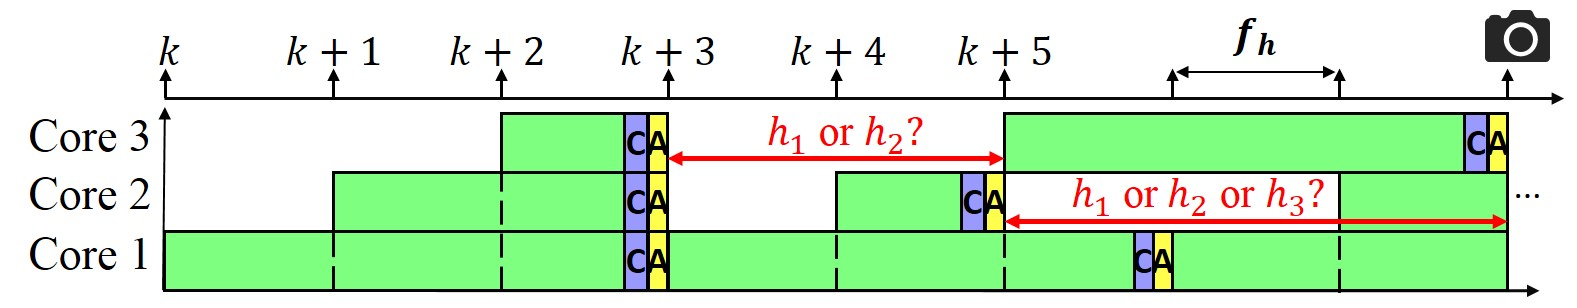
\includegraphics[width=0.95\textwidth]{images/pipeChallenge.jpg}
    %\vspace{-1em}
    \caption{Challenges in pipelined implementation due to switching when $h_i$ is a multiple of $\fh$. 
            }
    \label{fig:ch7_pipeChallenge}
   \vspace{-1em}
\end{figure}

Arbitrary switching and reconfiguration in the pipelined implementation are challenging.
Let $\numPipes$ be the number of pipes, and $h_s$ be the periods per system scenario. 
If we restrict $h_s$ to be a multiple of $\fh$, the number of periods possible due to arbitrary switching considering image-workload variations only grows linearly with $\fh$ and $\numPipes$.
However, if we do not restrict $h_s$ and allow it to take arbitrary values, the number of periods possible grows exponentially.
E.g. assume that we have three periods $h_1\ (=\ \fh$ for workload $\aWorkload_1),\ h_2\ (=\ 2\fh$ for workload $\aWorkload_2),$ and $h_3\ (=\ 3\fh$ for workload $\aWorkload_3)$ due to image-workload variations.
For simplicity, let us assume that $\tau_s=h_s$ and a given three-core platform allocation with three pipes. Consider the case shown in Fig.~\ref{fig:ch7_pipeChallenge} where the image frames $k,\ k+1, \dots,\ k+i$ have workload $\aWorkload_3,\ \aWorkload_2,\ \aWorkload_1,\ \aWorkload_3,\ \aWorkload_1,\ \aWorkload_3,$ and so on. When multiple control computations complete at the same time, e.g., just before frame $k+3$ is captured, the actuation should be coordinated among the cores.
Further, the controller for the image frame $k+4$ should ideally be designed using the discretized model considering $h_1=\fh$ if the period is defined as the time between two consecutive starts of the sensing task. However, it should also take into account that there was no actuation just before this, i.e., the previous actuation was at the time $t-2\fh$. So, if the period was defined as the time between two consecutive actuations, then the period for the controller for the frame at $k+4$ is $2\fh$.
A similar situation exists for frame $k+5$.
Such behaviours add to the complexity of the design space to be explored.
The main challenge, however, is proving the stability of the ensuing switched system with these behaviours.
Also, modelling these behaviours for the control design is far from trivial. 

For the scope of this work, we enforce a constant sampling period $h_\mathit{eff}$ for the overall pipelined implementation.
A constant sampling period helps to limit the design space to be explored and handle the dynamic reconfiguration with less runtime overhead.
As explained, the sensor-to-actuator delay $\tau_s$ is  constant per identified system scenario $\sysScenario$. Consequently, two system scenarios $s_1$ and $s_2$ have the control timing parameters $(h_\mathit{eff},\tau_1)$ and $(h_\mathit{eff},\tau_2)$.

A similar challenge exists for a pipelined implementation with resource sharing between pipes, where reconfiguring the mapping dynamically is non-trivial. 
Resource sharing between pipes increases the design space to be explored for considering the possible reconfiguration options. 
For the scope of this work, dynamic reconfiguration for pipelined implementation with resource sharing between pipes comprises a static mapping where actors are switched on and off considering image workload variations, and choosing the controller gains dynamically from the \gls{lut} by the control-computation task based on the system scenario considering the latest state measurement available.

The \gls{spade} flow is not restricted to the mentioned design and implementation choices. Its key feature is that pipelining and parallellism are integrally considered. As we will see, this provides benefits in the achievable QoC. Other controller design and implementation choices can be integrated as long as appropriate timing analysis and stability guarantees can be provided.